\documentclass{article}
\usepackage[utf8]{inputenc}
\usepackage{amsmath}
\usepackage[margin = 1in]{geometry}
\usepackage{listings}
\usepackage{fancyhdr}
\usepackage{graphicx}
\usepackage{listings}

\lstset{
	literate={~} {$\sim$}{1},
	belowcaptionskip=1\baselineskip,
	breaklines=true,
	frame=L,
	xleftmargin=\parindent,
	language=R,
	showstringspaces=false,
	basicstyle=\ttfamily
}

\pagestyle{fancy}
\fancyhead[L]{Variable Selection Techniques}
\fancyhead[R]{G. Ackall, C. Shrader}
\fancyfoot{}
\fancyfoot[C]{\thepage}

\setlength{\parskip}{6pt}

\title{Variable Selection Techniques}
\author{Gabriel Ackall and Connor Shrader}
\date{\today}

\newcommand{\argmin}{\text{arg min}}

\begin{document}
\maketitle

In mathematical modeling, especially when using linear regression, it is often important to reduce the number of predictors, or variables, used to predict an output. This can help to increase the interpretability of a model and reduce its error. Below are five methods used to select a linear model using a subset of the predictors.
% might need to add more here in the future


\section{Subset Selection}
\subsection{Best Subset Selection}
Best subset selection is a method for selecting the most influential predictors that minimize error in a least squares linear regression. It does this by fitting a linear regression model to every possible combination of predictors and then choosing the best model of all the possible combinations. The best model is determined through the use of a test error estimate. The most common examples of test error estimation indicators are Akaike information criterion (AIC), Bayesian information criterion (BIC), Adjusted $R^2$, and cross validation.

While best subset selection results in the best possible model given the predictors, it is very computationally expensive. As the number of predictors increases, the number of linear models that best subset selection has to fit increases exponentially. This can be seen in Table \ref{tab:subset-combinations}. Thus, for models with more than 40 predictors, this can become infeasible for most computers to compute \cite{james2013introduction}. Given that in many scenarios, especially those seen in medicine with genomic data or in scenarios where there are more predictors than data samples, there can be many thousands of predictors, and best subset selection becomes impossible.

\begin{table}[h!]
	\centering
	\caption{Number of fitted models depending on number of predictors (p)}
	\vspace{0.1in}
	\begin{tabular}{c|r@{\hskip 4pt}l}
		\hline
		p  &  \multicolumn{2}{c}{Fitted Models}\\
		\hline
		2   & $2^2$ & $=4$ \\
		10  & $2^{10}$ & $=1024$ \\
		100 & $2^{100}$ & $>10^{30}$ \\
		k   & $2^k$ & \\
	\end{tabular}
\label{tab:subset-combinations}
\end{table}

Figure \ref{fig:best-subset-selection} below demonstrates how the number of predictors can affect $R^2$ and BIC when using best subset selection. This plot was created by using the \lstinline!leaps! library (which provides a function to run best subset selection) \cite{lumley2020leaps}. We used the \lstinline!College! dataset provided by the \lstinline!ISLR! library \cite{james2017islr}, and fit linear regression models using \lstinline!Grad.Rate! as the response. We see that as the number of predictors increases, $R^2$ always increases (as expected). On the other hand, BIC is minimized with a moderate number of variables (between seven and nine). According to the BIC statistic, the best model has seven variables. The code used for this figure is in the \lstinline!r! folder of the REU GitHub repository.

\begin{figure}[!h]
	\label{fig:best-subset-selection}
	\centering
	\caption{$R^2$ and BIC when applying best subset selection}
	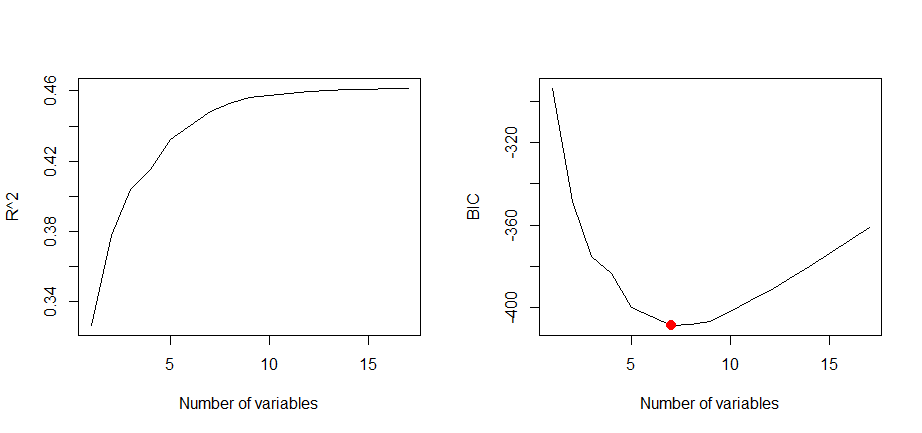
\includegraphics[width = 6in]{best-subset-selection.png}
\end{figure}

\subsection{Forward Stepwise Selection}
Forward stepwise selection aims to approximate the best combination of predictors in a linear regression model, but with a more computationally efficient method than best subset selection. Forward stepwise selection starts without using any predictors. It then slowly begins adding the most important predictor to the model. The predictor is chosen to minimize statistics such as p-value, AIC, BIC, or Adjusted $R^2$, to name a few. This is repeated until a stopping point is reached which can be defined by p-value, AIC, BIC, and more.

This process is much more computationally efficient than best subset selection, but it does not necessarily result in the best combination of parameters in the linear regression and is not guaranteed to result in the best model.

Figure \ref{fig:forward-stepwise-selection} shows the $R^2$ and BIC statistics when fitting models using forward stepwise selection. Again, we predicted \lstinline!Grad.Rate! using the \lstinline!College! data set using the \lstinline!leaps! library. The results are almost identical to what we saw for best subset selection. Even though the plots are similar, the specific model chosen by forward stepwise selection is actually different than the one found using best subset selection.

\begin{figure}[!h]
	\label{fig:forward-stepwise-selection}
	\centering
	\caption{$R^2$ and BIC when applying forward stepwise selection}
	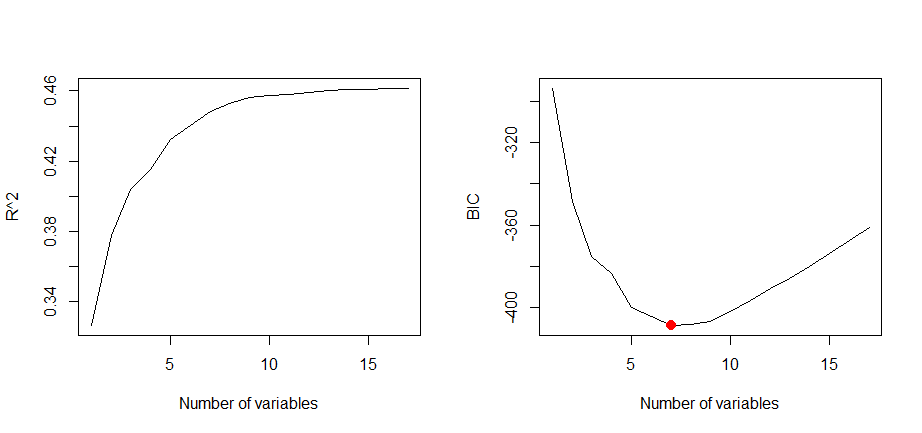
\includegraphics[width = 6in]{forward-stepwise-selection.png}
\end{figure}

\subsection{Backward Stepwise Selection}
Backwards stepwise selection works very similarly to forward stepwise selection, except that it starts with every single predictor included in the least squares linear regression. Instead of adding predictors like in forward stepwise selection, backward stepwise selection removes the least important predictor in each iteration. Similar to the forward method, the importance of a predictor can be determined by its p-value, AIC, BIC, or Adjusted $R^2$. This is repeated until a pre-determined stopping point is reached.

Backward stepwise selection can often result in better models than forward stepwise selection because it is guaranteed to test all the predictors together. This is different from forward stepwise selection that can sometimes suppress predictors, especially those that are collinear. For these reasons, when its use is possible, backward stepwise selection is preferred to forward stepwise selection. However, in cases where the number of predictors are greater than the number of samples, backward stepwise selection is impossible. In these case, forward stepwise selection must be used.

Figure \ref{fig:backward-stepwise-selection} shows $R^2$ and BIC after applying backward stepwise selection to the \lstinline!College! data set. Again, the results are very similar to Figures \ref{fig:best-subset-selection} and \ref{fig:forward-stepwise-selection}, but the particular models chosen by the algorithm were slightly different. 

\begin{figure}[!h]
	\label{fig:backward-stepwise-selection}
	\centering
	\caption{$R^2$ and BIC when applying backward stepwise selection}
	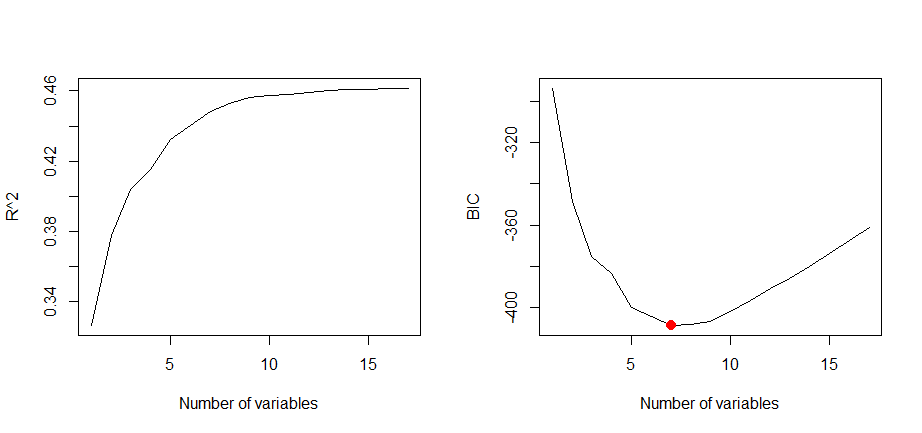
\includegraphics[width = 6in]{backward-stepwise-selection.png}
\end{figure}

\subsection{Hybrid Stepwise Selection}
One weakness of the forward stepwise and backward stepwise methods is that they are greedy algorithms; in general, they will not find the best model for a given number of predictors. One way to improve model accuracy is to use hybrid stepwise selection, which allows for both forward steps and backward steps \cite{friedman2001elements}.

The algorithm could start with either zero predictors or all predictors. In each iteration, the method would either add a new predictor to the model or remove a predictor that does not increase performance. Like the forward and backward stepwise selection methods, this algorithm terminates when the model cannot be improved further; measuring the accuracy of the model can be determined using the AIC or BIC.

Although this strategy is slightly more computationally expensive than forward stepwise or backward stepwise selection, a hybrid approach may improve model results while still avoiding the unrealistic runtime of best subset selection.

\subsection{Forward Stagewise Selection}
One last method for feature selection is called forward stagewise regression. Like forward stepwise selection, forward stagewise selection starts by fitting a model using none of the predictors. In each iteration, the method chooses the predictor most closely correlated to the residuals of the current model, and fits a simple linear regression using the predictor against the residuals. The coefficient for this predictor in the simple model is then added to the corresponding coefficient in the other model. This process is repeated until none of the predictors are correlated with the residuals.

Note that in each iteration of this algorithm, only one of the coefficients is changed. As a result, this method has a long runtime. In the long run, forward stagewise selection is still competitive compared to the strategies previously discussed.

\section{Penalized Regression}
\subsection{Ridge Regression}
Ridge regression helps to solve multicollinearity in predictors while also minimizing insignificant predictors. While it does not minimize these insignificant predictors completely to 0 and thus cannot be considered a variable selection method, it still proves very useful in large datasets.

Ridge regression works by minimizing Residual Sum Squared (RSS) plus a penalty as seen in Equation \ref{ridge_reg}. $\lambda$ is a tuning parameter and can be used to determine how much of an effect the penalty has on the regression. if $\lambda=0$, then the regression acts exactly like ordinary least squares regression, but if $\lambda \rightarrow \infty$, then $\beta_j \rightarrow 0$ and the regression line will only be $\beta_0$.

\begin{equation}
	\hat{\beta}^{\text{ridge}} = \argmin\left\{ \sum_{i=1}^{n} \left( y_i - \beta_0 - \sum_{j=1}^{p} \beta_jx_{ij} \right)^2 + \lambda \sum_{j=1}^{p} \beta_j^2 \right\}
	\label{ridge_reg}
\end{equation}

\subsection{Lasso Regression}

The least absolute shrinkage and selection operation, often referred to as \textit{lasso}, is a shrinkage method with a very similar form to lasso regression. The coefficient estimates satisfy
\begin{equation}
	\hat{\beta}^{\text{lasso}}=\argmin\left\{ \sum\limits_{i = 1}^n \left( y_i - \beta_0 - \sum\limits_{i = 1}^p \beta_j x_{ij} \right) + \lambda\sum\limits_{j = 1}^p \vert \beta_j \vert \right\}
\end{equation}
Unlike ridge regression, the lasso is able to perform variable selection.

\subsection{Elastic Net Regression}

\subsection{Adaptive Lasso}

\subsection{Smoothly Clipped Absolute Deviation Regression}

\subsection{Multiple Change Points Regression}

\bibliographystyle{plain}
\bibliography{references}
\end{document}
